%priprava posamezne ure
%tukaj zaporedoma napisemo{st. zaporedne ure}{datum}{naslov}{poglavje}{oblika dela}{pripomocki}
\begin{priprava}{}{}{Odvod}{Odvodi drugih elementarnih funkcij}{frontalna}{tabla}

\didopomba{Do sedaj smo odvajali le polinome in racionalne funkcije.}

\textbf{Odvod sestavljene funkcije}

Vemo že: $ (x^5)' = 5 \cdot x^4 $. Koliko pa je $ ((2x + 1)^5)' $?

Spomnimo se kopozituma: $ (g \circ f)(x) = g(f(x)) $

\textcolor{red}{$ (g \circ f)'(x) = g'(f(x)) \cdot f'(x) $} \didopomba{dokaz v učb., ne bi ga med poukom}

Primer $ ((2x + 1)^5)': f(x) = 2x + 1 \rightarrow f'(x) = 2, g(x) = x^5 \rightarrow g'(x) = 5 x^4 $. Zato je $ ((2x + 1)^5)' = 5 (2x + 1)^4 \cdot 2 = 10 (2x + 1)^4 $

Oz. $ (\square ^n)' = n \cdot \square^{n - 1} \cdot \square' $.

\vaje{Vaje: razne potence polinomov, korenske funkcije \ldots}

\textbf{Odvod trigonometrijskih funkcij}

Ponovimo pomembne lastnosti, ki nam pomagajo pri izpeljavi odvodov:
\begin{itemize}
    \item $ \sin^2 x + \cos^2 x = 1 $
    \item $ \sin(\frac{\pi}{2} - x) = \cos x $ in $ \cos(\frac{\pi}{2} - x) = \sin x $
    \item $ \lim_{x \to 0} \frac{\sin x}{x} = 1 $
    \item $ \sin \alpha - \sin \beta = 2 \cos \frac{\alpha + \beta}{2} \sin \frac{\alpha - \beta}{2} $
    \item $ \tan x = \frac{\sin x}{\cos x} $ in $ \cot x = \frac{\cos x}{\sin x} $
\end{itemize}

\didopomba{Začnemo dokazovati za $ \sin $, ki je najtežji, ostali sledijo iz tega. Lahko dokažemo pri pouku (gl. učbenik)}

\textcolor{red}{
    $ (\sin x)' = \cos x \\ (\cos x)' = - \sin x \\ (\tan x)' = \frac{1}{\cos^2 x} \\ (\cot x)' = - \frac{1}{\sin^2 x} $
}

\didopomba{Tu je argument $ x $ v radianih -- če je v stopinjah, imamo sestavljeno funkcijo: $ (\sin (x\text{°}))' = cos(\frac{x\text{°}}{360\text{°}} 2\pi) \cdot (\frac{x\text{°}}{360\text{°}} 2\pi)' = cos(x\text{°}) \cdot \frac{\pi}{180\text{°}} $}

\vaje{Vaje iz teh funkcij, tudi že sestavljene npr.
\begin{itemize}
    \item $ (\sin^2 x)', (x^5 \cdot \sin {7x})' $ \ldots
    \item Gasilci so poklicani v intervencijo v bolnišnico, kjer je hodnik dimenzije kot na sliki. S seboj želijo vzeti najdaljšo možno lestev, ki bo še šle čez ovinek. Kako dolgo lestev lahko vzamejo?
\newpage
    \begin{figure*}[h]
        \centering
        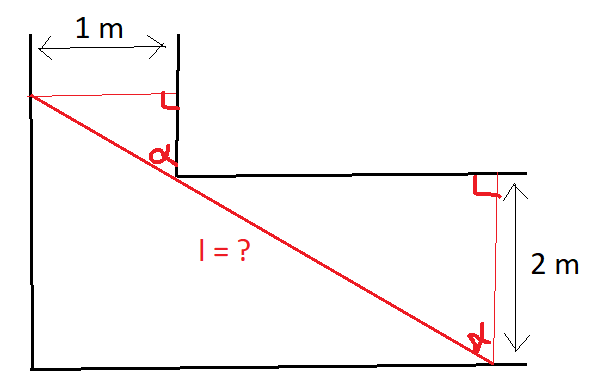
\includegraphics[width=0.4\textwidth]{slike/ekstremproblem.png}
    \end{figure*}
$ l(\alpha) = \frac{1}{\sin \alpha} + \frac{2}{\cos \alpha} $, odvajaš in rešuješ $ l'(\alpha) = 0 $ in za izračunani $ \alpha $ je rezultat $ f(\alpha) $.   
\end{itemize}
}

\textbf{Odvod inverzne funkcije}

Vemo $ (g \circ f)'(x) = g'(f(x)) \cdot f'(x) $
\begin{align*}
    (f \circ f^{-1})(x) = f(f^{-1}(x)) & = x \\
    (f \circ f^{-1})'(x) & = x' \\
    f'(f^{-1}(x)) \cdot (f^{-1}(x))' & = 1 \\
\end{align*}
Sledi $ \textcolor{red}{(f^{-1}(x))' = \frac{1}{f'(f^{-1}(x))}} $

Zdaj lahko odvajamo tudi krožne funkcije:

$ (\arcsin x)' = \frac{1}{\cos (\arcsin x)} = \frac{1}{\sqrt{1 - \sin^2 (\arcsin x)}} = \frac{1}{\sqrt{1 - x^2}}  \\
(\arccos x)' = \frac{1}{- \sin (\arccos x)} = - \frac{1}{\sqrt{1 - \cos^2 (\arccos x)}} = - \frac{1}{\sqrt{1 - x^2}} \\
(\arctan x)' = \frac{1}{\frac{1}{\cos^2 \arctan x}} = \cos^2 \arctan x = \frac{1}{\sqrt{1 + \tan^2 (\arctan x)}} = \frac{1}{1 + x^2} \\
(arccot x)' = \frac{1}{\frac{1}{- \sin^2 arccot x}} = - \sin^2 arccot x = - \frac{1}{\sqrt{1 + \cot^2 (arccot x)}} = - \frac{1}{1 + x^2} $

\textbf{Odvod logaritemske in eksponentne funkcije}

\textcolor{red}{
    $ (\log_a x)' = \frac{1}{x \cdot \ln a} $ \didopomba{po definiciji, gl. učbenik ALI pa najprej izpeljemo za $ \ln $ in navaden logaritem zapišemo z novo osnovo. Saj ni važno.} \\
    $ (\ln x)' = \frac{1}{x} $ \didopomba{to sledi iz zgoraj za $ a = e $} \\
    $ (a^x)' = a^x \cdot \ln a $ \didopomba{po formuli za odvod inverzne funkcije}\\
    $ (e^x)' = e^x $ \didopomba{to sledi iz zgoraj za $ a = e $}
}

\vaje{funkcijo $ \ln |x| $ se spozna (funkcijo $ \ln x $ se samo preslika še na desno stran), in jo lahko odvajamo na vsaki strani osi, v obeh primerih dobiš odvod enak $ 1/x $ ne glede na predznak $ x $.}

\textbf{Odvod implicitno podane funkcije}

Imejmo krožnico s polmerom $ r = 2 $ in središčem v $ S(0, 0) $. Točka $ A $ ima $ x $-koordinato 1 in leži v 1. kvadrantu. Kakšen je koeficient tangente na krožnico, ki gre skozi točko $ A $? Kakšna je njena enačba? \didopomba{rešimo na 3 načine}
\begin{enumerate}
    \item Koeficient izračunamo preko pravokotnice na tangento (daljica od izhodišča do $ A $)
    \item Koeficient izračunamo, da odvajamo enačbo krožnice, kjer smo izrazili $ y $ (ker je $ A $ na zgodnji polovici, vzamemo pri korenu predznak +)
    \item Enačbo $ x^2 + y^2 = 4 $ odvajamo kot sestavljeno funkcijo (pri tem je $ y $ odvisen od $ x $, torej na $ y $ ne gledamo samo kot na spremenljivko, ampak kot funkcijo) $ \rightarrow 2x + 2 y y' = 0 \rightarrow y' = - \frac{x}{y} $, vstaviš noter $ A $ in dobiš.
\end{enumerate}

\vaje{podobne vaje}
    
\end{priprava}